\section{Metodología de Trabajo}\label{sec:metodologiaDeTrabajo}

\subsection{Ciclo de vida} 

Teniendo en cuenta las características del proyecto y las características del equipo se decidió utilizar un ciclo de vida 
incremental.  Dado que el conocimiento en el dominio y en las tecnologías utilizadas por el cliente nos permiten poder obtener 
al principio del proyecto la definición de los requerimientos y la arquitectura.

El proyecto se dividió en dos etapas:

\textbf{Discovery.}\\
Utilizando la metodología \textit{Design Thinking} y el marco de gestión Kanban con el objetivo de relevar los requerimientos a ser ejecutados 
en los primeros \textit{sprint} y también para definir la arquitectura durante un \textit{sprint} 0 en los meses de abril, mayo y junio. 

\textbf{Delivery.}\\
Para cada iteración de duración fija de dos semanas entre los meses de julio a diciembre realizaremos el diseño, codificación y pruebas de forma 
incremental adaptando el marco de gestión \textit{scrum}.

Se utilizará la metodología \textit{Dual Track Scrum} con algunas adaptaciones, porque entendemos que algunos requerimientos podrían requerir de actividades 
de \textit{discovery} durante el proyecto. Se evaluó utilizar solamente \textit{scrum} pero se decidió complementar el inicio generando un primer \textit{backlog} para 
alimentar sus iteraciones con una primera fase de \textit{discovery} a fin de mejorar la Ingeniería de Requerimientos.


\subsubsection{Discovery} \\
Durante la etapa de Discovery, el equipo optó por utilizar el marco de gestión Kanban para la organización y seguimiento de las tareas relacionadas con el marco
de ingeniería de Design Thinking. Durante el Sprint 0, se elaboró un backlog inicial de funcionalidades basado en las necesidades identificadas. Posteriormente, 
se tomaron decisiones de arquitectura que fueron validadas por expertos en la materia, asegurando así que las soluciones propuestas fueran viables y alineadas con 
los objetivos del proyecto.\\
La elección del marco Kanban fue estratégica, dado que permite una visualización clara y dinámica del flujo de trabajo. Cada columna del tablero Kanban se 
correspondió con una etapa del ciclo Design Thinking, lo que facilitó la organización y priorización de las tareas a lo largo del sprint. Esta metodología es particularmente 
útil en entornos donde se requiere flexibilidad y adaptación continua, características inherentes al proceso de Design Thinking.\\
Para llevar a cabo esta gestión, se utilizó la herramienta Trello, seleccionada debido a la experiencia previa del equipo con la misma. Trello proporciona una interfaz intuitiva 
que facilita la colaboración y el seguimiento en tiempo real del progreso de las tareas, permitiendo a todos los miembros del equipo estar al tanto del estado actual de cada actividad y 
realizar ajustes en tiempo real si es necesario.\\

\begin{figure}[H]
    \centering
    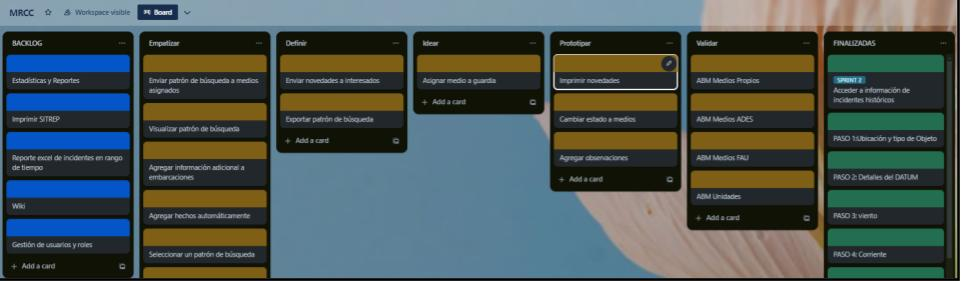
\includegraphics[width=0.8\textwidth]{../imagenes/secciones/3-marco-metodologico/Tablero Kanban de tareas de la etapa de discovery.jpg}
    \caption{Tablero Kanban utilizado durante la etapa de Discovery}
    \label{fig:kanbanDiscovery}
\end{figure}

Finalmente, a medida que las tareas avanzaban y se completaban, se refinó el backlog, el cual servirá como base para la etapa de Delivery. Este enfoque no solo garantizó una 
alineación efectiva entre el diseño y la ejecución, sino que también permitió al equipo mantenerse ágil y receptivo a los cambios y descubrimientos que surgieron durante la 
etapa de Discovery.\\

\subsubsection{Delivery} \\
Para la etapa de Delivery, se adoptó el marco Scrum, estableciendo sprints de duración fija de 2 semanas. Esta decisión se fundamentó en la disponibilidad continua de nuestro cliente, 
quien realizaba guardias de 24 horas al menos una vez cada dos semanas. Esto brindó una oportunidad ideal para realizar el Sprint Review durante su turno, asegurando una retroalimentación 
oportuna y precisa.\\

\textit{Sprint planning}\\
El Sprint Planning se llevó a cabo el primer día de cada sprint, con la participación de todo el equipo. Este evento fue crucial para la planificación del trabajo a realizar durante la 
iteración y, por tanto, no se incluyó al cliente en esta fase. El proceso comenzó con la selección de las Historias de Usuario que serían abordadas en el sprint. Luego, el equipo se organizó 
para descomponer estas historias en tareas técnicas específicas. Para gestionar y hacer el seguimiento del sprint, se utilizó la herramienta Azure DevOps, lo que permitió una planificación detallada 
y un monitoreo efectivo del progreso.

\textit{Daily meeting}\\
Para mantener una comunicación fluida y abordar cualquier impedimento que surgiera durante el sprint, se informó diariamente a través de un grupo de WhatsApp del equipo. Este método aseguró una 
respuesta rápida a cualquier obstáculo que pudiera retrasar el avance. Además, el equipo se reunió semanalmente mediante videollamada para coordinar el progreso y discutir dudas que fueron planteadas 
en la reunión semanal con el cliente. Esta estructura de comunicación permitió resolver problemas de manera ágil y aseguró que el equipo estuviera alineado con los objetivos del sprint.

\textit{Sprint reviewg}\\
El Sprint Review se realizó idealmente el penúltimo día de cada sprint. Sin embargo, se intentó ajustar la agenda para coincidir con un turno de guardia del cliente, aprovechando así su disponibilidad 
para una revisión más exhaustiva. En esta reunión, se enfocó exclusivamente en las tareas que fueron completadas durante el sprint, recogiendo feedback del cliente. Para maximizar la utilidad de la 
retroalimentación, se grabaron las reuniones, lo que permitió que el equipo se concentrará en el diálogo y luego documentará los puntos clave a partir de la grabación. Este enfoque aseguró que las 
observaciones del cliente fueran capturadas de manera precisa y pudieran ser integradas en las siguientes iteraciones.

\textit{Sprint retrospective}\\
La Sprint Retrospective se llevó a cabo el último día de cada sprint, con la participación de todo el equipo. Similar al Sprint Planning, este evento no incluyó al cliente, ya que su objetivo fue 
interno: reflexionar sobre el desempeño del equipo durante el sprint. Se utilizó la herramienta DAKI para estructurar la retrospectiva, identificando qué se hizo bien, qué se podría mejorar, y qué 
se debía evitar o continuar en las próximas iteraciones. Esta práctica fue fundamental para la mejora continua del equipo y para garantizar que cada sprint fuera más eficiente que el anterior.

\textit{Sprint backlog}\\
El Sprint Backlog fue una lista de las tareas que el equipo se comprometió a completar durante el sprint. Se actualizó continuamente a medida que el equipo avanzaba en sus tareas, reflejando el 
progreso real y permitiendo ajustes según fuera necesario. Utilizar Azure DevOps para gestionar el Sprint Backlog proporcionó una plataforma robusta para la planificación y seguimiento, asegurando 
que el equipo se mantuviera enfocado y que las prioridades se gestionaron de manera efectiva.\\
El sprint board fue configurado de la siguiente manera:\\


\begin{itemize}
    \item \textbf{To Do:} Listado de tareas prontas para ser iniciadas
    \item \textbf{Develop:} Tareas que se encuentran en desarrollo por un miembro del equipo y que antes de pasar a la próxima etapa deberán ser sometidas a la revisión cruzada de código.
    \item \textbf{QA:} Tareas que se encuentran prontas para hacer pruebas funcionales manuales por otro miembro del equipo.
    \item \textbf{Done:} Tareas completadas.
\end{itemize}

\begin{figure}[H]
    \centering
    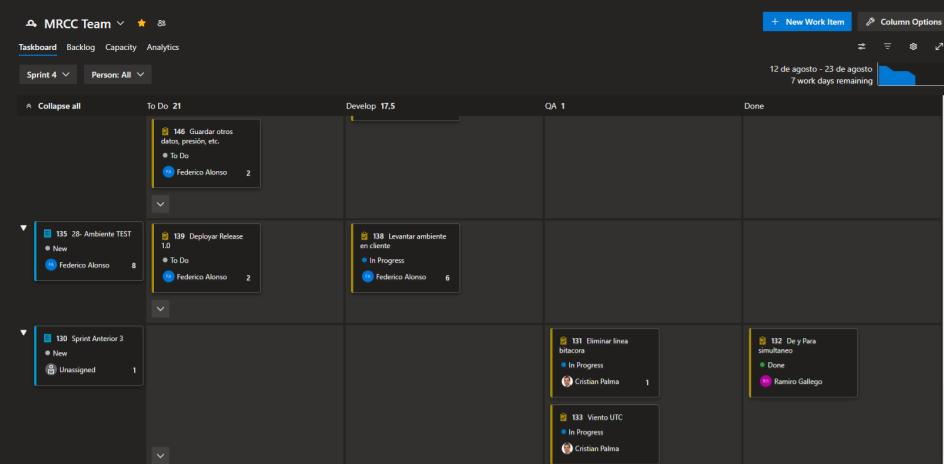
\includegraphics[width=0.8\textwidth]{../imagenes/secciones/3-marco-metodologico/Sprint Board.jpg}
    \caption{Tareas del Sprint Board}
    \label{fig:sprintBoard}
\end{figure}

Este enfoque estructurado y justificado en cada aspecto del marco Scrum permite no solo cumplir con los plazos establecidos, sino también asegurar una calidad constante en la entrega del producto 
final, alineando los esfuerzos del equipo con las expectativas del cliente.\\

\textit{Reuniones semanales con tutor}\\
Además de los eventos regulares de Scrum, durante todo el proyecto se llevaron a cabo reuniones semanales con nuestro tutor, Juan Pablo Russo. Estas sesiones fueron fundamentales, ya que nos 
proporcionaron orientación en diversas áreas, como la gestión del proyecto, las estimaciones de esfuerzo, la definición del alcance, y la organización del equipo, entre otros aspectos clave. 
En cada una de estas reuniones se elaboraron minutas, lo que permitió realizar un seguimiento exhaustivo del equipo y de las tareas y recomendaciones planteadas por el tutor.



\textit{Herramientas utilizadas}\\
Para la gestión de tareas y el seguimiento del progreso, se utilizaron las siguientes herramientas:
\begin{itemize}
    \item \textbf{Azure DevOps:} Para la planificación y seguimiento de los sprints, así como para la gestión del código fuente y la integración continua.
    \item \textbf{Clockify:} Para el seguimiento del tiempo dedicado a cada tarea y la generación de informes de productividad.
    \item \textbf{Google Docs:} Para la elaboración de documentos colaborativos, como minutas de reuniones y otros documentos de trabajo.
    \item \textbf{WhatsApp:} Para la comunicación diaria y la resolución de problemas urgentes.
    \item \textbf{DAKI:} Para la realización de retrospectivas y la identificación de mejoras en el proceso.
    \item \textbf{Trello:} Para la organización y seguimiento de las tareas durante la etapa de Discovery.
    \item \textbf{Microsoft Teams:} Para la realización de reuniones semanales con el tutor y la comunicación interna del equipo.
    \item \textbf{Google Meets:} Para la realización de reuniones con el cliente y la comunicación interna del equipo.
    \item \textbf{GitHub:} Para el control de versiones del código fuente y la colaboración en el desarrollo.
    \item \textbf{Postman:} Para la realización de pruebas de integración y pruebas de API.
    \item \textbf{Docker:} Para la creación de contenedores y la gestión de la infraestructura.
    \item \textbf{Latex:} Para la documentación y la colaboración en la creación de documentos.
    \item \textbf{PostgreSQL:} Para la gestión de la base de datos y la persistencia de los datos.
    \item \textbf{React:} Para la creación de interfaces de usuario y la interacción con el usuario.
\end{itemize}


\textit{Roles del equipo}\\
A lo largo de la carrera y de experiencia laboral, nuestro equipo cuenta con varias capacidades generales. La dinámica de tésis forzará a que nuestro equipo trabaje en estrecha colaboración implicando 
que compartimos conocimientos, resolvamos problemas conjuntamente y tomamos decisiones de manera colectiva pero de tomas maneras se opta por designar un referente para cada una de las siguientes áreas:

\begin{itemize}
    \item \textbf{Arquitectura de software:} Federico Alonso
    \item \textbf{Gestión de proyecto:} Cristian Palma
    \item \textbf{Ingeniería de requerimientos:} Cristian Palma
    \item \textbf{Gestión de calidad:} Horacio Ábalos
    \item \textbf{UX/ UI:} Ramiro Gallego
    \item \textbf{Gestión de riesgos:} Horacio Ábalos
    \item \textbf{Gestión de configuración:} Federico Alonso
    \item \textbf{Desarrollo:} Todo el equipo
    \item \textbf{Pruebas:} Todo el equipo
    \item \textbf{Documentación:} Todo el equipo
    \item \textbf{Presentación:} Todo el equipo
    \item \textbf{Reuniones con el cliente:} Todo el equipo
    \item \textbf{Reuniones con el tutor:} Todo el equipo
    \item \textbf{Reuniones internas:} Todo el equipo
    \item \textbf{Reuniones de retrospectiva:} Todo el equipo
    \item \textbf{Reuniones de planificación:} Todo el equipo
    \item \textbf{Reuniones de revisión:} Todo el equipo
    \item \textbf{Reuniones diarias:} Todo el equipo
    \item \textbf{Reuniones de seguimiento:} Todo el equipo
\end{itemize}

Como equipo de scrum, cada miembro del equipo tiene un rol específico y se espera que cumpla con las responsabilidades asociadas a ese rol. Los roles asignados son los siguientes:

\begin{itemize}
    \item \textbf{Product Owner:} Cristian Palma
    \item \textbf{Scrum Master:} Horacio Ábalos
    \item \textbf{Development Team:} Todo el equipo
\end{itemize}